\section{Minimal Axioms of Intelligence}

\subsection{Overview}

\S{}2 positioned intelligence as ongoing motion that produces stopping structures without becoming one. This section formulates the minimal structural conditions under which such motion can persist.

The aim is not to define intelligence completely. The aim is to formulate a lower bound. A dynamic system that lacks any of the following conditions is unlikely to sustain intelligence-like dynamics in the sense used here. Conversely, a system that satisfies all three conditions possesses the minimal structure required for the kind of ongoing motion described in \S{}2.

The axioms are intentionally minimal. Meaning, purpose, judgment, correctness, agency, and subjectivity are not introduced at the axiomatic level. They may appear later as interpretive projections or higher-layer structures, but they are not required for the structural onset of intelligence-like dynamics.

\subsection{Axiom I: Connected state space}

The first axiom is the existence of a connected state space.

Let the set of possible states be
\[
\mathcal{S}=\{s_1,s_2,\dots\}.
\]
Connectedness means that states are not merely listed. They must stand in direct or indirect relations of transition, influence, or dependence.

This does not require a continuous topology. A discrete graph is sufficient, provided that states can be reached through some chain of transitions. Without connectedness, information cannot propagate or accumulate. The system reduces to a collection of isolated reactions rather than a single dynamical system.

\subsection{Axiom II: Temporal ordering}

The second axiom is temporal ordering. State updates must occur in an order, and prior states must constrain later states. Abstractly,
\[
s(t+1)=F(s(t)).
\]
The specific form of $F$ is not fixed by the axiom.

Temporal ordering does not require an external clock. What is required is that updates are not purely simultaneous and that change leaves some trace. This is consistent with the differential-development structure of VED \citep{VEDVol1}: past differences become part of the generated texture on which later differences operate.

Without temporal ordering, a connected state space under a global bias collapses toward static fixation. It may have an optimal state, but it lacks motion.

\subsection{Axiom III: Global constraint $\Phi$}

The third axiom is the existence of a global constraint $\Phi$. Formally,
\[
\Phi:\mathcal{S}\rightarrow\mathbb{R}.
\]
\(\Phi\) biases the dynamics of the system as a whole.

\(\Phi\) is not purpose, meaning, value, or normativity. It is a structural bias. It directs state transitions and prevents uncontrolled diffusion, but it does not decide what is correct.

\(\Phi\) is not reducible to a simple aggregation of local update rules. This is its central role. Even if every local transition is well-defined, the absence of a global constraint leaves the system directionless. Conversely, the presence of $\Phi$ produces a global consistency that cannot be derived from local rules alone.

Different systems instantiate $\Phi$ differently. In physical systems it may appear as a potential, Hamiltonian, or entropy function. In biological systems it may appear as nutrient gradients, boundary conditions, or metabolic constraints. In artificial systems it may appear as a loss function, reward structure, or training distribution.

\subsection{The joint necessity of the three axioms}

No single axiom is sufficient.

If Axiom I is absent, the system becomes a collection of isolated local optimizers. If Axiom II is absent, the system freezes into static fixation. If Axiom III is absent, the system becomes an unbounded reaction or memory process without global direction.

\begin{table}[H]
\centering
\small
\begin{tabularx}{\textwidth}{>{\raggedright\arraybackslash}X>{\raggedright\arraybackslash}X>{\raggedright\arraybackslash}X}
\toprule
Missing axiom & Degenerate form & Example \\
\midrule
I: connectedness & isolated local optimization & parallel independent reactors \\
II: temporal ordering & static fixation & frozen optimization problem \\
III: global constraint & directionless diffusion & random walk with memory \\
\bottomrule
\end{tabularx}
\end{table}

Only their simultaneous satisfaction produces the minimal form of ongoing motion described in \S{}2. This is the paper's minimal definition of intelligence-like dynamics.

\subsection{Semantic neutrality of the axioms}

The three axioms do not presuppose semantic content, purpose, correctness, agency, or subjectivity. These concepts may appear later, but they are not part of the lower-bound structure.

This neutrality makes cross-domain comparison possible. A slime mold network, a Transformer, a biological organism, and a social process may differ radically in substrate, but they can still be examined for the same structural conditions.

\subsection{Summary}

\begin{quote}
Intelligence is not an ability or possession. It is a dynamical state that can persist only under structural conditions. Those conditions are the simultaneous satisfaction of connected state space, temporal ordering, and a global constraint $\Phi$.
\end{quote}

These axioms form a lower bound, not an upper bound. A system satisfying them is not necessarily highly intelligent. A system lacking them cannot sustain the kind of intelligence-like motion considered here.

\begin{figure}[H]
\centering
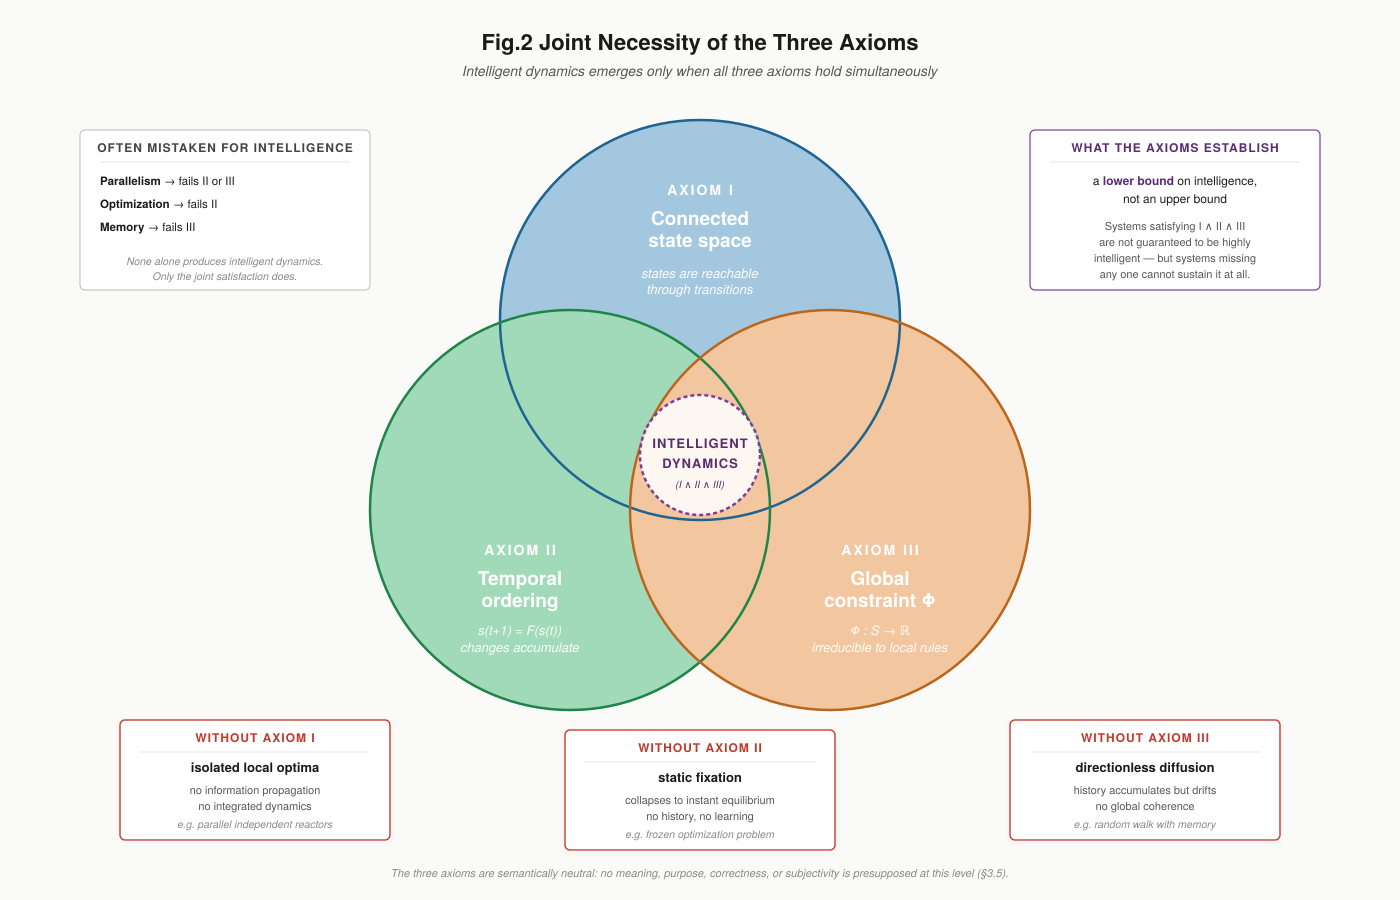
\includegraphics[width=\textwidth]{figures/fig2_three_axioms.png}
\caption{Joint necessity of the three axioms. Intelligence-like dynamics appears only where connected state space, temporal ordering, and a global constraint hold together.}
\label{fig:intelligence_part1_2}
\end{figure}
